% label C_\pm on fig 2
% unify 3 & 4, choose consistent q/cos q

% S2: CS stability
% S3: How to reach CS
% S3: toy problem, affords analytical understanding
% S4: full problem
% Discussion/conclusion: maybe 0.05 AU + SE? does this still work?
    \documentclass[
        fleqn,
        usenatbib,
        % referee,
    ]{mnras}
    \usepackage{
        amsmath,
        amssymb,
        newtxtext,
        newtxmath,
        ae, aecompl,
        graphicx,
        booktabs,
        xcolor,
    }

    \newcommand*{\scinot}[2]{#1\times10^{#2}}
    \newcommand*{\rd}[2]{\frac{\mathrm{d}#1}{\mathrm{d}#2}}
    \newcommand*{\rtd}[2]{\frac{\mathrm{d}^2#1}{\mathrm{d}#2^2}}
    \newcommand*{\pd}[2]{\frac{\partial#1}{\partial#2}}
    \newcommand*{\ptd}[2]{\frac{\partial^2#1}{\partial#2^2}}
    % inline
    \newcommand*{\mdil}[2]{\mathrm{D}#1/\mathrm{D}#2}
    \newcommand*{\pdil}[2]{\partial#1/\partial#2}
    \newcommand*{\rdil}[2]{\mathrm{d}#1/\mathrm{d}#2}
    \newcommand*{\at}[1]{\left.#1\right|}
    \newcommand*{\abs}[1]{\left|#1\right|}
    \newcommand*{\ev}[1]{\left\langle#1\right\rangle}
    \newcommand*{\p}[1]{\left(#1\right)}
    \newcommand*{\s}[1]{\left[#1\right]}
    \newcommand*{\z}[1]{\left\{#1\right\}}
    \newcommand*{\bm}[1]{\mathbf{#1}}
    \newcommand*{\uv}[1]{\hat{\mathbf{#1}}}
    \newcommand*{\md}[0]{\mathrm{d}}
    \DeclareMathOperator*{\med}{med}
    \DeclareMathOperator*{\erf}{erf}

\title[Weak Tides and Cassini States]{Dynamics of Colombo's Top: Tidal
Dissipation and Resonance Capture}
\author[Y. Su and D. Lai.]{
Yubo Su,$^1$\thanks{E-mail: yubosu@astro.cornell.edu},
Dong Lai$^{1,2}$
\\
$^1$ Cornell Center for Astrophysics and Planetary Science, Department of
Astronomy, Cornell University, Ithaca, NY 14853, USA\\
$^2$ Tsung-Dao Lee Institute \& School of Physics and Astronomy, Shanghai Jiao
Tong University, 200240 Shanghai, China
}

\date{Accepted XXX\@. Received YYY\@; in original form ZZZ}

\pubyear{2021}

\begin{document}\label{firstpage}
\pagerange{\pageref{firstpage}--\pageref{lastpage}}
\maketitle

\begin{abstract}
    Abstract here
\end{abstract}

\begin{keywords}
planet-star interactions
\end{keywords}

\section{Introduction}

\begin{itemize}
    \item Studying planetary obliquities (define) is important. Cassini States
        are key. More introduction.

    \item Resonance capture via separatrix crossing was first considered by
        \citep{henrard1982} for non-dissipative perturbations
        \citep[e.g.][]{su2020}. However, tidal friction is dissipative, so this
        formalism does not apply. We generalize this calculation and show that
        it reproduces results.
\end{itemize}

In Section XXX\dots

\section{Spin Evolution Equations and Cassini States: Review}\label{s:theory}

In this section, we first briefly lay out the spin dynamics of the planet,
introducing the Cassini State spin-orbit resonance \citep[for more details,
see][]{su2020}. We then introduce the weak friction theory of equilibrium tides
used in this work \citep{lai2012}. While many different tidal effects may
dominate in different planetary systems, our qualitative conclusions do not
depend on the specific form of the tidal dissipation, so we use the classic weak
friction theory for simplicity.

\subsection{Spin Dynamics in the Absence of Tides}\label{ss:theory_spin}

\subsubsection{Equations of Motion}

We consider a star of mass $M_\star$ hosting an inner oblate planet of mass $m$
and radius $R$ on a circular orbit with semi-major axis $a$ and an outer
perturber of mass $m_{\rm p}$ on a circular orbit with semi-major axis $a_{\rm
p}$. We assume that the two orbits are mildly misaligned with mutual inclination
$I$. Denote $\bm{S}$ the spin angular momentum and $\bm{L}$ the orbital angular
momentum of the planet, and $\bm{L}_{\rm p}$ the angular momentum of the
perturber. The corresponding unit vectors are $\uv{s} \equiv \bm{S} / S$,
$\uv{l} \equiv \bm{L} / L$, and $\uv{l}_{\rm p} \equiv \bm{L}_{\rm p} / L_{\rm
p}$. The spin axis $\uv{s}$ of the planet tends to precess around its orbital
(angular momentum) axis $\uv{l}$, driven by the gravitational torque from the
host star acting on the planet's rotational bulge. On the other hand, $\uv{l}$
and the disk axis $\uv{l}_{\rm p}$ precess around each other due to
gravitational interactions. We assume $S \ll L \ll L_{\rm p}$, so $\uv{l}_{\rm
p}$ and $\uv{l}$ are nearly constant. The equations of motion for $\uv{s}$ and
$\uv{l}$ in this limit are \citep{anderson2018teeter, su2020}
\begin{align}
    \rd{\uv{s}}{t}
        &= \omega_{\rm sl}\p{\uv{s} \cdot \uv{l}}\p{\uv{s} \times \uv{l}}
        \equiv \alpha\p{\uv{s} \cdot \uv{l}}\p{\uv{s} \times
        \uv{l}},\label{eq:dsdt1}\\
    \rd{\uv{l}}{t} &= \omega_{\rm lp}\p{\uv{l} \cdot \uv{l}_{\rm p}}\p{\uv{l}
        \times \uv{l}_{\rm p}} \equiv -g\p{\uv{l} \times \uv{l}_{\rm p}},
        \label{eq:dldt1}
\end{align}
where
\begin{align}
    \omega_{\rm sl} &\equiv \frac{3GJ_2 mR^2 M_\star}{2a^3 I\Omega_{\rm s}}
        = \frac{3k_q}{2k}\frac{M_\star}{m}\p{\frac{R}{a}}^3 \Omega_{\rm s},
            \label{eq:wsl}\\
    \omega_{\rm lp} &= \frac{3m_p}{4M_\star}\p{\frac{a}{a_{\rm p}}}^3
        n.\label{eq:wlp}
\end{align}
In Eq.~\eqref{eq:wsl}, $\Omega_{\rm s}$ is the spin frequency of the inner
planet, $I = k mR^2$ (with $k$ a constant) is its moment of inertia and $J_2 =
k_{\rm q}\Omega_{\rm s}^2 (R^3/Gm)$ (with $k_{q}$ a constant) is its rotation-induced
(dimensionless) quadrupole moment [for a body with uniform density, $k=0.4,
k_{\rm q}=0.5$; for rocky planets, $k\simeq 0.2$ and $k_{\rm q}\simeq 0.17$
\citep[e.g.][]{lainey2016quantification} \textcolor{red}{? not sure}]. In other
studies, $3k_{\rm q} / 2 k$ is often notated as $k_2 / 2C$
\citep[e.g.][]{millholland_disk}. In Eq.~\eqref{eq:wlp}, $n \equiv
\sqrt{GM_\star/a^3}$ is the inner planet's orbital mean motion,  and we have
assumed $a_{\rm p}\gg a$ and included only the leading-order (quadrupole)
interaction between the inner planet and perturber. Following standard notation,
we define $\alpha = \omega_{\rm sl}$ and $g \equiv -\omega_{\rm 1p} \cos I$
\citep[e.g.][]{colombo1966}.

As in \citet{su2020}, we combine Eqs.~(\ref{eq:dsdt1}--\ref{eq:dldt1}) into a
single equation by transforming into a frame rotating about $\uv{l}_{\rm p}$
with frequency $g$. In this frame, $\uv{l}_{\rm p}$ and $\uv{l}$ are both fixed,
and $\uv{s}$ evolves as:
\begin{equation}
    \p{\rd{\uv{s}}{t}}_{\rm rot}
        = \alpha\p{\uv{s} \cdot \uv{l}}\p{\uv{s} \times \uv{l}}
            + g\p{\uv{s} \times \uv{l}_{\rm p}}. \label{eq:dsdt_rot}
\end{equation}
In this reference frame, we choose the coordinate system such that $\uv{z} =
\uv{l}$ and $\uv{l}_{\rm p}$ lies in the $\uv{x}$-$\uv{z}$ plane. We describe
$\uv{s}$ in spherical coordinates using the polar angle $\theta$, the planet's
obliquity, and $\phi$, the precessional phase of $\uv{s}$ about $\uv{l}$.

The equilibria of Eq.~\eqref{eq:dsdt_rot} are referred to as \emph{Cassini
States} \citep[CSs;][]{colombo1966, peale1969}. We follow the notation of
\citet{su2020}, where the parameter
\begin{equation}
    \eta \equiv -\frac{g}{\alpha},\label{eq:def_eta}
\end{equation}
is used. For a given value of $\eta$, there can be either two or four CSs, all
of which require $\uv{s}$ lie in the plane of $\uv{l}$ and $\uv{l}_{\rm p}$.
Following the standard convention and nomenclature, CSs 1, 3, and 4 have $\phi =
0$ and $\theta < 0$, while CS2 has $\phi = \pi$ and $\theta > 0$.
Figure~\ref{fig:cs_locs} shows the CS obliquities as a function of $\eta$, each
of which satisfies
\begin{equation}
    \sin \theta \cos \theta - \eta \sin\p{\theta - I} = 0.\label{eq:cs_zero}
\end{equation}
Note that there are four CSs when $\eta < \eta_{\rm c}$ and only two when $\eta
> \eta_{\rm c}$, where
\begin{equation}
    \eta_{\rm c} \equiv \p{\sin^{2/3}\!I + \cos^{2/3}\!I}^{-3/2}.\label{eq:etac}
\end{equation}
\begin{figure}
    \centering
    %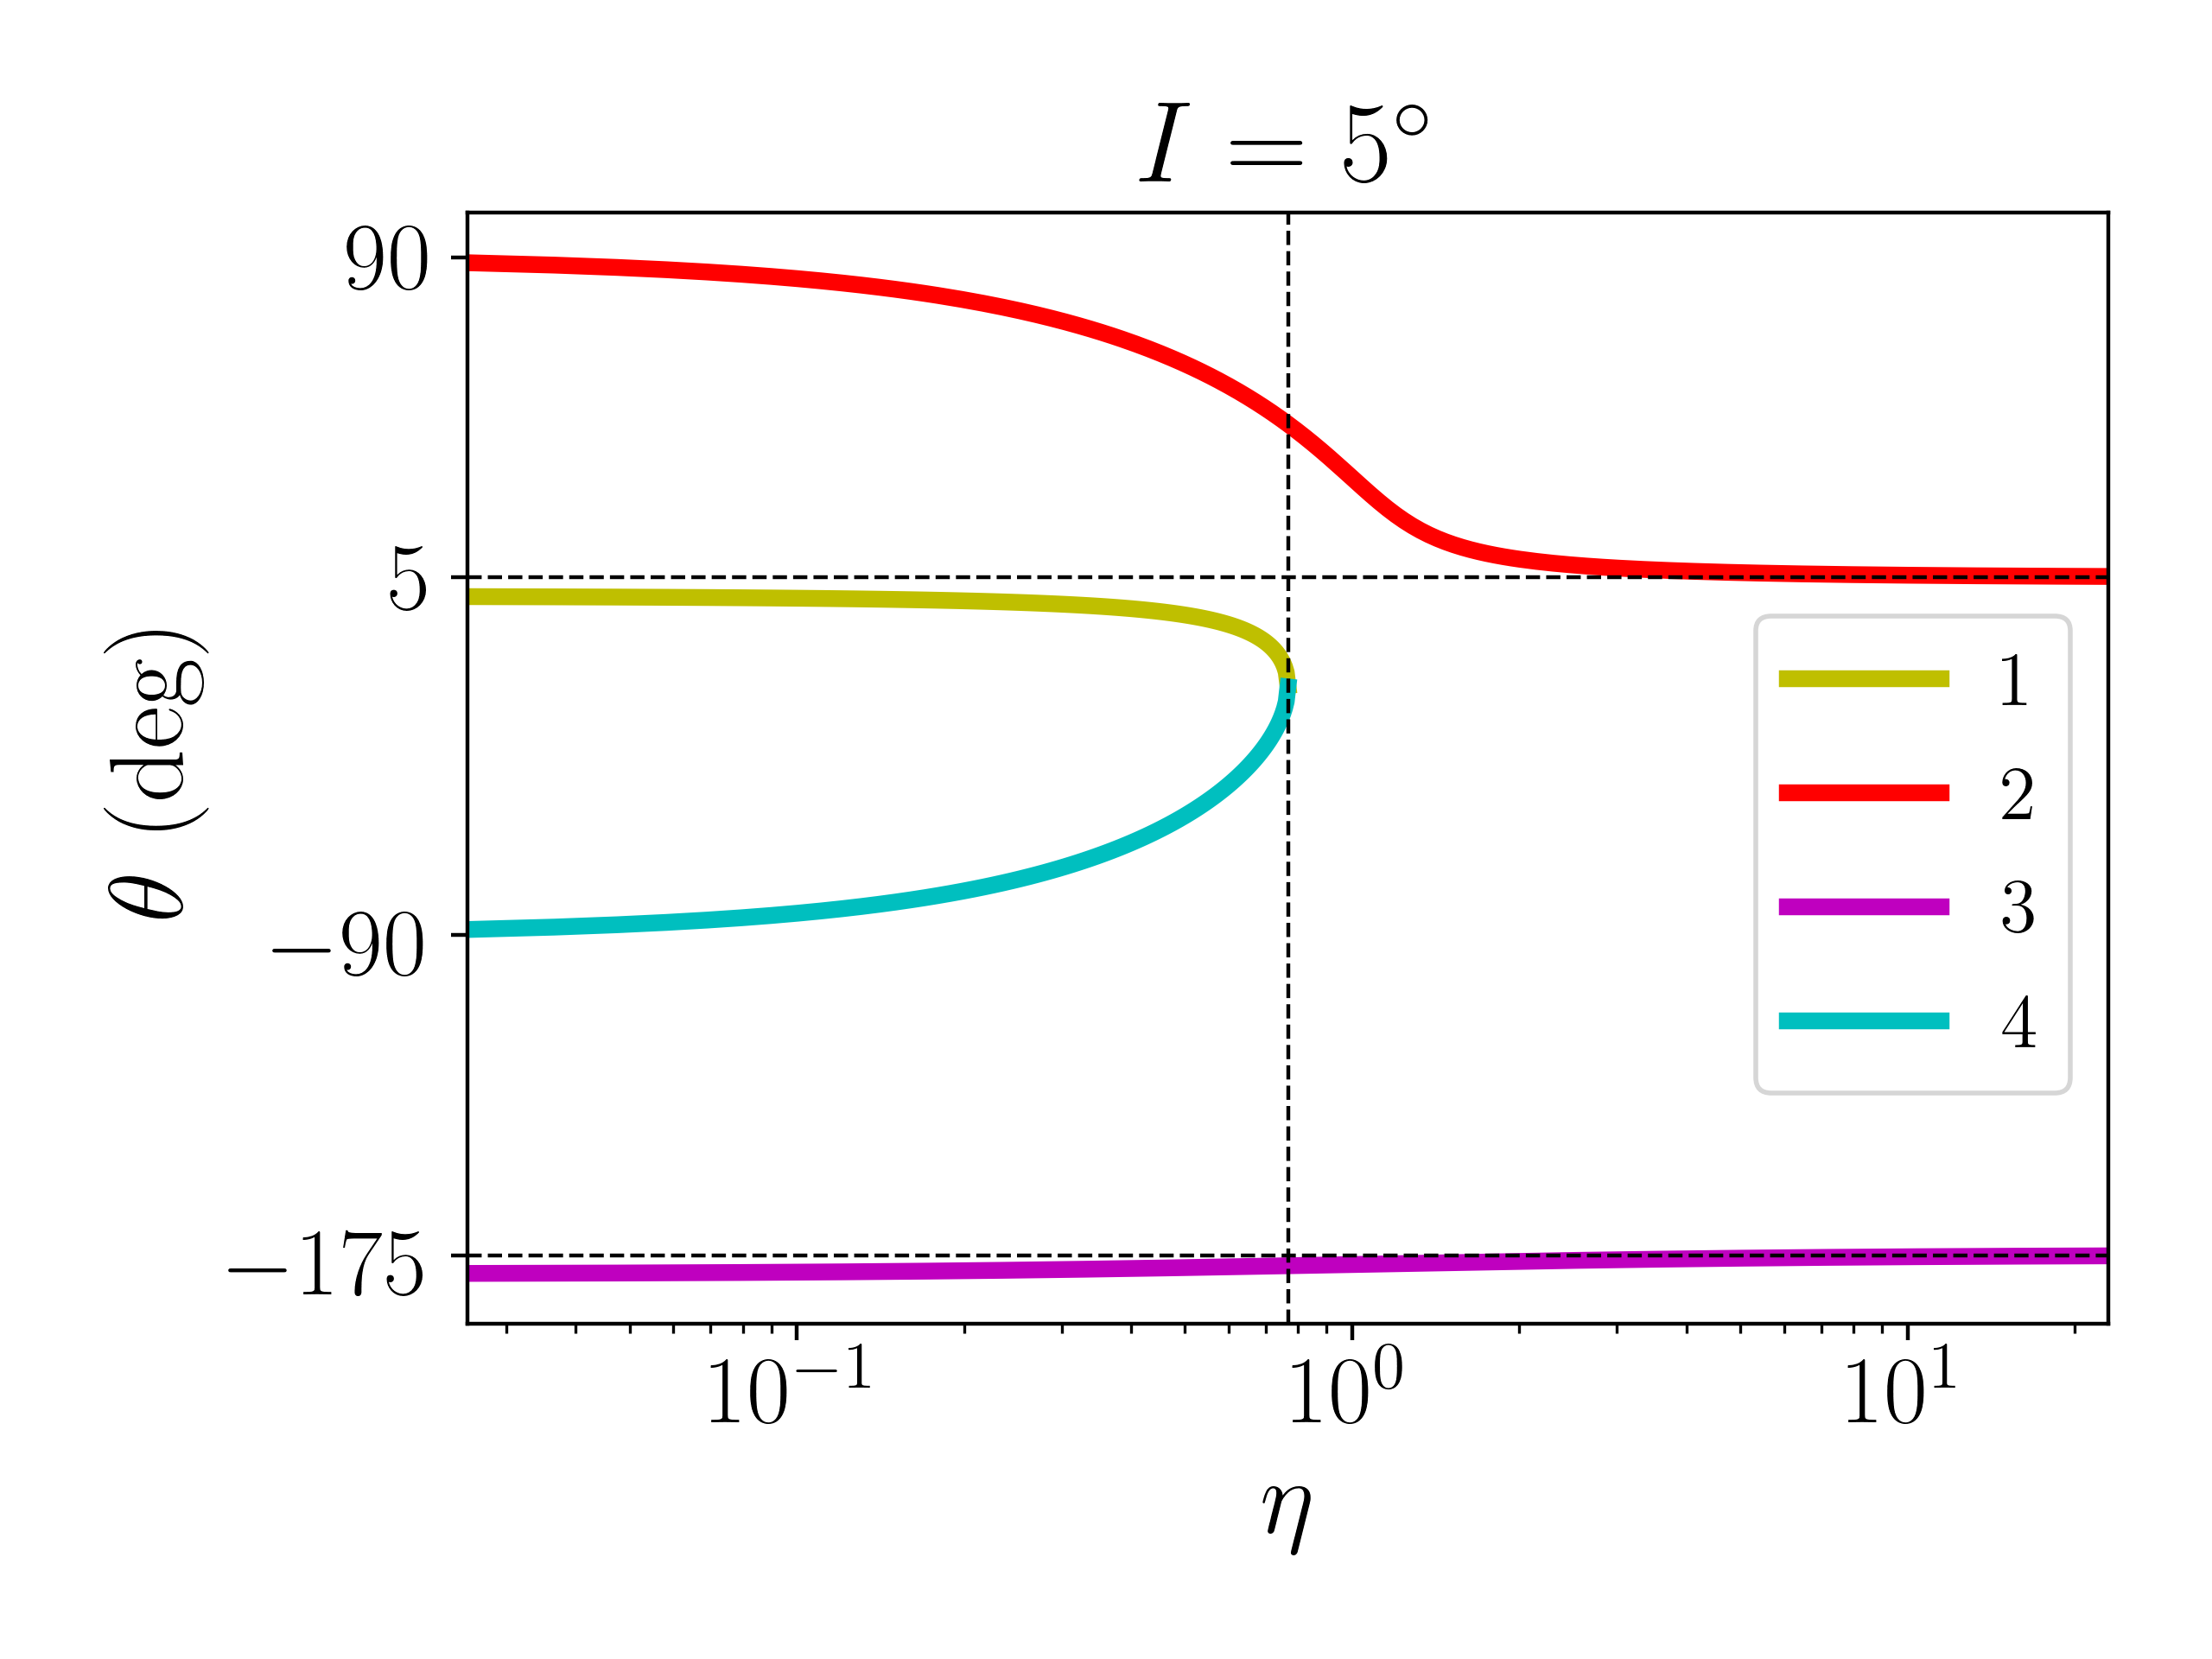
\includegraphics[width=\columnwidth]{../initial/99_misc/2_cs_locs.png}
    \caption{Cassini State obliquities $\theta$ as a function of $\eta \equiv
    -g/\alpha$ (Eq.~\ref{eq:def_eta}) for $I = 5^\circ$. The vertical dashed
    line denotes $\eta_{\rm c}$, where the number of Cassini States changes from
    four to just two (Eq.~\ref{eq:etac}). The horizontal dashed line gives
    $\theta = I$, the asymptotic value of Cassini State 2's obliquity when $\eta
    \to \infty$.}\label{fig:cs_locs}
\end{figure}

The Hamiltonian corresponding to Eq.~\eqref{eq:dsdt_rot} is
\begin{align}
    H &= -\frac{\alpha}{2}\p{\uv{s} \cdot \uv{l}}^2
            - g\p{\uv{s} \cdot \uv{l}_{\rm d}}\nonumber\\
        &= -\frac{\alpha}{2} \cos^2\theta
            - g\p{\cos\theta \cos I - \sin I \sin\theta \cos \phi}.\label{eq:H}
\end{align}
Here, $\cos \theta$ and $\phi$ form a canonically conjugate pair of variables.
Figure~\ref{fig:1contours} shows the level curves of this Hamiltonian for $I =
20^\circ$, for which $\eta_{\rm c} \approx 0.77$ (Eq.~\ref{eq:etac}). When $\eta
< \eta_{\rm c}$, CS4 exists and is a saddle point. The two trajectories
originating and ending at CS4 are the only two infinite-period orbits in the
phase space. Together, these two critical trajectories are referred to as the
\emph{separatrix} and divide phase space into three zones. Trajectories in zone
II librate about CS2 while those in zones I and III circulate. On the other
hand, when $\eta > \eta_{\rm c}$, all trajectories circulate. When the
separatrix exists, we divide it into two curves: $\mathcal{C}_+$, the boundary
between zones I and II, and $\mathcal{C}_-$, the boundary between zones II and
III\@.
\begin{figure}
    \centering
    %\includegraphics[width=\columnwidth]{../initial/0_eta/1contours.png}
    \caption{Level curves of the Cassini State Hamiltonian (Eq.~\ref{eq:H}) for
    $I = 5^\circ$, for which $\eta_{\rm c} \approx 0.77$ (Eq.~\ref{eq:etac}).
    For $\eta < \eta_{\rm c}$, there are four Cassini States (labeled), while
    for $\eta > \eta_{\rm c}$ there are only two. In the former case, the
    existence of a \emph{separatrix} (solid black lines) separates phase space
    into three numbered zones (I/II/III, labeled). Finally, we denote the upper
    and lower legs of the separatrix by $\mathcal{C}_{\pm}$ respectively, as
    shown in the upper two panels.}\label{fig:1contours}
\end{figure}

\section{Spin Evolution with Alignment Torque}\label{ss:toy_model}

In this section, we consider a simplified model of equilibrium tides that
isolates the important new phenomenon presented in this paper. We assume that
the spin magnitude of the planet is constant, so $\alpha$ and $g$ are both
fixed, while the spin orientation $\uv{s}$ experiences a torque that drives it
towards alignment with $\uv{l}$ on the alignment timescale $t_{\rm s}$:
\begin{equation}
    \p{\rd{\uv{s}}{t}}_{\rm tide}
        = \frac{1}{t_{\rm s}} \uv{s} \times \p{\uv{l} \times \uv{s}}.
\end{equation}
The full equations of motion for $\uv{s}$ in the coordinates $\theta$ and $\phi$
can be written:
\begin{align}
    \rd{\theta}{t} &= -g\sin I \sin \phi - \frac{1}{t_{\rm s}} \sin \theta,
        \label{eq:dqdt_toy}\\
    \rd{\phi}{t} &= -\alpha \cos\theta
        - g\p{\cos I + \sin I \cot \theta \cos \phi}.\label{eq:dfdt_toy}
\end{align}

\subsection{Shifted Cassini States and Linear Stability
Analysis}\label{ss:tidal_eqs}

When $t_{\rm s}$ is finite, the CSs tilt out of the $\uv{l}$-$\uv{l}_{\rm p}$
plane \citep[as was first pointed out for CS2 by][]{fabrycky_otides}. A simple
expression for the degree of this tilt can be obtained by solving for $\phi_{\rm
cs}$, the azimuthal angle of the modified CS, when setting Eq.~\eqref{eq:dqdt_toy} equal
to zero. This gives
\begin{equation}
    \sin \phi_{\rm cs} = \frac{\sin^2\theta_{\rm cs}}{\sin I \abs{g}t_{\rm s}}.
\end{equation}
Here, $\theta_{\rm cs}$ is the modified CS obliquity. Note that if $t_{\rm s}$
is shorter than some critical value $t_{\rm s, c}$, which for a given CS is
given by
\begin{align}
    t_{\rm s, c} &= \frac{\sin^2\theta_{\rm cs}}{\abs{g}\sin I},
\end{align}
then there are no solutions for $\phi_{\rm cs}$, and the CS is no longer a fixed
point. This condition first breaks down for $\theta_{\rm cs} \approx 90^\circ$,
i.e.\ for CS2 (and CS4) in the limit $\eta \ll 1$. Thus, as long as $t_{\rm s}
\gtrsim \p{\abs{g}\sin I}^{-1}$, then all CSs will exist.

We next seek to characterize the stability of small perturbations about each of
the CSs in the presence of the alignment torque. We can linearize
Eqs.~(\ref{eq:dqdt_toy}--\ref{eq:dfdt_toy}) about a [modified] CS, yelding
\begin{align}
    \rd{}{\tau}\begin{bmatrix}
        \theta\\ \phi
    \end{bmatrix} &= \begin{bmatrix}
        -\frac{\cos \theta}{t_{\rm s}} &
        -g\sin I \cos \phi \\
        \alpha \sin \theta + g\frac{\sin I \cos \phi}{\sin^2\theta} &
        0
    \end{bmatrix}_{\rm cs}\begin{bmatrix}
        \Delta \theta \\ \Delta \phi
    \end{bmatrix},\label{eq:dsdt_hessian}
\end{align}
where the cs subscript indicates evaluating at a CS, $\Delta \theta = \theta -
\theta_{\rm cs}$, and the same for $\Delta \phi$. The eigenvalues $\lambda$ of
Eq.~\eqref{eq:dsdt_hessian} satisfy the equation
\begin{align}
    0 &= \p{\lambda + \frac{\cos \theta_{\rm cs}}{t_{\rm s}}}\lambda - \lambda_0^2,\\
    \lambda_0^2 &\equiv \p{\alpha
        \sin \theta_{\rm cs} + g\sin I \csc^2\theta_{\rm cs}\cos \phi_{\rm cs}}
            \p{- g \sin I \cos \phi_{\rm cs}},\\
    \lambda &\approx -\frac{\cos \theta_{\rm cs}}{t_{\rm s}} \pm \sqrt{\lambda_0^2}.
        \label{eq:lambda_approx}
\end{align}
The stability depends only on the real part of
$\lambda$ in Eq.~\eqref{eq:lambda_approx}. If we assume that the torque-induced
modification to $\phi_{\rm cs}$ is small, then $\lambda_0$ reduces to the
product of the eigenvalues in the torque-free limit. In this limit, $\lambda_0^2
< 0$ for each of CSs 1--3 and $\lambda_0^2 > 0$ for CS4 \citep[see Fig.~17
of][]{su2020}. Thus, CS4 is always unstable, since there will always be a
positive eigenvalue $\lambda$, while the stability of CSs 1--3 are solely
determined by the sign of $\cos \theta_{\rm cs}$. From Fig.~\ref{fig:cs_locs},
we see that CSs 1 and 2 are stable while CS3 is unstable under the alignment
torque. These calculations justify results long used in CS literature
\citep[e.g.][]{ward1975tidal}.

\subsection{Spin Obliquity Evolution Driven by Alignment Torque}

With the above results, we are equipped to ask the key question of this section:
for a given initial $\theta_0$ and $\phi_0$, which of CS1 and CS2 does the
system evolve into? For initial conditions in Zone I (see
Fig.~\ref{fig:1contours}), an unperturbed trajectory circulates and returns to
$(\theta_0, \phi_0 + 2\pi)$ after a single precession period. During this
period, the effect of the dissipation is a negative $\theta'$ everywhere during
the cycle. Thus, for initial conditions in Zone I, $\theta$ decreases until the
trajectory has converged to CS1. This is intuitively reasonable, as CS1 is
stable. For initial conditions in Zone II, an equivalent calculation to that in
Section~\ref{sss:cs_stab2} shows that all trajectories converge to CS2.

For illustrative purposes, we fix $\abs{g}t_{\rm s} = 10^{-3}$, and $\eta =
-g / \alpha$ is varied among a few small values (small
meaning much less than $\eta_{\rm c}$). We specialize to the case where $\eta
< \eta_{\rm c}$ and there are four CSs.

However, initial conditions in Zone III pose a puzzle. There are no stable CSs
in Zone III, so the system must evolve through the separatrix to reach one of
either CS1 or CS2. In Fig.~\ref{fig:toy_phop}, we find see that the outcome for
initial conditions in Zone III is in fact \emph{probabilistic}. Intuitively,
this can be understood as probabilistic resonance capture: since $\eta \ll
\eta_{\rm c}$, $\alpha \gg -g$ (the spin-orbit precession rate,
Eq.~\ref{eq:dsdt1}, and the orbit precession induced by the perturber,
Eq.~\ref{eq:dldt1}, respectively), but $\alpha \cos \theta$ can become
commensurate with $-g$ if $\cos \theta \sim \eta$. This is achieved as $\theta$
evolves from an initially retrograde obliquity through $90^\circ$ towards
$0^\circ$ under the influence of the dissipative term in
Eq.~\eqref{eq:dqdt_toy}.
\begin{figure}
    \centering
    %\includegraphics[width=\columnwidth]{../initial/0_eta/3stats3_5_0_2.png}
    \caption{TODO generate a better plot. Ignore bottom two panels, top two
    panels show which ICs end up in CS 1 (left) and CS2 (right). Probabilistic
    behavior in Zone III is evident.}\label{fig:toy_phop}
\end{figure}

While similar in behavior to previous studies of probabilistic resonance capture
\citep{henrard1982, su2020}, the mechanism at play here is necessarily
different: here, the Hamiltonian and underlying phase structure is kept constant
while a non-Hamiltonian, dissipative perturbation is introduced. The origin of
this resonance crossing process is easy to visualize. In the absence of
dissipative effects, the separatrix is both the set of points that flow into CS4
and the set of points that flow away CS4, called the \emph{stable} and
\emph{unstable} manifolds of the saddle point CS4 respectively \citep{g_and_h}.
When the dissipative term is taken into account, these stable and unstable
manifolds split and open a visible ``path'' from Zone III into both Zones I and
II, as shown in Fig.~\ref{fig:toy_hop_manifolds}.
\begin{figure}
    \centering
    %\includegraphics[width=\columnwidth]{../initial/0_eta/6manifolds0_05.png}
    \caption{TODO overplot separatrix, remove bad labels, better legend. Stable
    and unstable manifolds of CS4, showing how the separatrix splrits and gives
    a ``path'' from Zone III into Zones I/II.}\label{fig:}
\end{figure}

The amount that the stable and unstable manifolds split can be calculated
perturbatively using \emph{Melnikov's Method} \citep{g_and_h}. The essence of
Melnikov's method lies at the heart of the perturbative approach used in
Section~\ref{sss:cs_stab2}, where the evolution of $H$ along the perturbed
trajectories can be evaluated by integration along their original
\emph{unperturbed} trajectories. In particular: \textcolor{red}{TODO the rest of
this section is copy pasted from notes without even notation changes, needs to
be written up correctly} Now, let's reconsider the Melnikov integral when
perturbing this finite (non-homoclinic orbit); this may no longer be an exact
result but should give the correct scaling:
\begin{equation}
    M_c = \int\limits_0^T \pd{\phi}{t}\epsilon \p{1 - \mu^2}\;\mathrm{d}t.
\end{equation}
Naively, we might claim that, since $\pd{\phi}{t}$ changes signs halfway through
the interval of integration, that the only surviving component is $2\epsilon
\bar{\mu}\mu'$, where $\bar{\mu} = \mu_4$ is the average value of $\mu$ and
$\mu'$ is the fluctuation. This gives
\begin{equation}
    M_c = 2\int\limits_0^{2\pi}2\epsilon \frac{\eta \cos I}{1 + \eta \sin I}
        \sqrt{2\eta \sin I \p{1 - \cos \phi}}\;\mathrm{d}\phi.
\end{equation}
Note that $M_c \propto \eta^{3/2}$, and since the gap opened $\Delta_c =
\frac{M_c}{\pd{\phi}{t}} \propto \eta$, it seems like we're on the right track.
Specifically:
\begin{align}
    M_c &\approx \epsilon 2\eta \cos I A_{sep},\\
    \Delta_c &\approx 2\epsilon \eta \cos I \p{16 \sqrt{\eta \sin I}}
        \frac{1}{\sqrt{4\eta \sin I}},\\
        &\approx 16\epsilon \eta \cos I.
\end{align}
This also agrees exceedingly well with our simulations This then gives us
hopping probability
\begin{equation}
    P_{hop} = \frac{\Delta_c}{\Delta_M} \approx
        \frac{16\eta^{3/2}\cos I \sqrt{\sin I}}{\pi}.
\end{equation}
This agrees perfectly with the cases we've run.

\textbf{Note:} The full formula, by actually evaluating all the terms, comes out
to be
\begin{equation}
    P_{hop} = \frac{16\eta^{3/2}\cos I \sqrt{\sin I}}{\pi
        \p{1 - 2\eta \sin I - \eta^2 \cos^2 I}
        + 8\eta^{3/2}\cos I \sqrt{\sin I}}.
\end{equation}

\section{Spin Evolution with Weak Tidal Friction}\label{ss:full_tide_prob}

\begin{figure}
    \centering
    %\includegraphics[width=\columnwidth]{../initial/1_weaktide/6equils0_06.png}
    \caption{Schematic illustrating the evolution of the planet's spin due to
    tidal friction. The green lines illustrate the directions of
    Eqs.~(\ref{eq:dsdt_tide}--\ref{eq:dWsdt_tide}), while the black and blue
    lines denote where the tidal $\Omega_{\rm s}'$ and $\theta'$ change signs
    respectively. Overlaid are the obliquities of Cassini States 1 and 2, the
    two Cassini States that are stable under tidal dissipation (see
    Section~\ref{ss:tidal_eqs}). The points that are both Cassini States and
    satisfy $\Omega_{\rm s}' = 0$ are the tidal Cassini Equilibria (tCE),
    circled in green. Finally, the vertical red lines illustrate the
    $\Omega_{\rm s}$ below which tides causes tCE2 to become unstable; the
    dashed and dotted lines correspond to values of $\epsilon = 10^{-2}$ and
    $10^{-1}$ respectively.
    }\label{fig:6equils}
\end{figure}

\subsection{Tidal Model: Equilibrium Tides}\label{sss:weaktide}

To model the dissipative effect of times, we use the weak friction theory of
equilibrium tides \citep{lai2012}. In this model, tides cause both $\uv{s}$ and
$\Omega_{\rm s}$ to evolve following:
\begin{align}
    \p{\rd{\uv{s}}{\tau}}_{\rm tide} &= \epsilon
                \s{\frac{2n}{\Omega_{\rm s}} - \p{\uv{s} \cdot \uv{l}}}
                    \uv{s} \times \p{\uv{l} \times \uv{s}}\label{eq:dsdt_tide},\\
    \frac{1}{\Omega_{\rm s}}\p{\rd{\Omega_{\rm s}}{\tau}}_{\rm tide}
        &= \epsilon \s{\frac{2n}{\Omega_{\rm s}}\p{\uv{s} \cdot
            \uv{l}} - \p{1 + \p{\uv{s} \cdot \uv{l}}^2}},\label{eq:dWsdt_tide}
\end{align}
where $\epsilon$ is the dimensionless tidal evolution rate, given by
\begin{align}
    \epsilon \equiv{}& -\frac{1}{gt_a}\frac{L}{2S} \frac{\Omega_{\rm s}}{2n},\\
        % = \frac{1}{\cos I} \frac{2k_2}{Q} \frac{n}{\Omega_{\rm c}},\\
    \frac{1}{t_a} ={}& \frac{3k_2}{Q}\p{\frac{m}{M}}\p{\frac{R}{a}}^5 n,\\
    \epsilon \approx{}& 0.003\frac{1}{\cos I}\p{\frac{2k_2/Q}{10^{-3}}}
            \p{\frac{m_{\rm p}}{M_{\rm J}}}^{-1}
            \p{\frac{a_{\rm p}}{5 \;\mathrm{AU}}}^{3}\nonumber\\
        &\times \p{\frac{a}{0.4\;\mathrm{AU}}}^{-6}
            \p{\frac{\rho}{3 \; \mathrm{g/cm}^3}}^{-1}
            \p{\frac{M_\star}{M_{\odot}}}^{2}.
\end{align}
Here, $L = ma^2n$ and $S = kmR^2 \approx mR^2/4$ are the orbital and spin
angular momenta of the inner planet, respectively. In Eq.~\eqref{eq:dsdt_tide},
it is clear that tides only acts on the polar component of $\uv{s}$,
i.e.\ $\theta$, and not the azimuthal component $\phi$. As such,
the effect of tides on the dynamics of the system can be qualitatively
understood in $(\Omega_{\rm s}, \theta)$ space. Figure~\ref{fig:6equils} shows
the behavior of Eqs.~(\ref{eq:dsdt_tide}--\ref{eq:dWsdt_tide}) in a few
characteristic regions of $(\Omega_{\rm s}, \theta)$ space.

Component form
\begin{align}
    \rd{\theta}{t} &= g\sin I \sin \phi -
        \epsilon \sin \theta,\label{eq:ds_fullq}\\
    \rd{\phi}{t} &= -\alpha\cos\theta
        - g\p{\cos I + \sin I \cot \theta \cos \phi}\label{eq:ds_fullphi},\\
    \rd{\Omega_{\rm s}}{t}
        &= \epsilon \s{2n \cos \theta
            - \Omega_{\rm s}\p{1 + \cos^2\theta}}\label{eq:ds_fulls}.
\end{align}

For the parameters considered here, the tidal evolution in $\Omega_{\rm s}$ and
$\theta$ occurs over characteristic time scale $2 \times 10^8\;\mathrm{yr}$.
Note that while the semimajor axis $a$ is not strictly constant under the
influence of tidal dissipation, $\dot{a} / \dot{\theta} \sim S / L \ll 1$
\citep{lai2012} and the evolution of $a$ can be safely neglected in this paper.

Armed with the intuition provided by the toy model in
Section~\ref{ss:toy_model}, we now study the equations of motion including the
full weak tidal friction theory, given by
Eqs.~(\ref{eq:ds_fullq}--\ref{eq:ds_fulls}). We imagine that the inner planet is
born rapidly spinning, but for computational reasons, we restrict the initial
spin to be $\Omega_{\rm s, i} = 10n$. The final results are not sensitive on the
specific initial spin as long as $\Omega_{\rm s, i} \gg n$. The hierarchy of the
system is determined by the parameter $\Omega_{\rm c}$, given by
Eq.~\eqref{eq:def_Wc}, for which we choose a few representative values. Then,
for a given initial $\theta_0$ and $\phi_0$, the final outcome (between tCE1 and
tCE2) of the system can
be calculated. In Fig.~\ref{fig:Hhists_0_06}, we show the final outcome for many
randomly chosen $\theta_0$ and $\phi_0$ for $\Omega_{\rm c} = 0.06$ and $I =
5^\circ$. We see that tCE1 is generally reached for spins initially in Zone I,
tCE2 is generally reached for spins initially in Zone II, and a probabilistic
outcome is observed for spins initially in Zone III, very similar to the results
found for the toy model in Section~\ref{ss:toy_model}.
Figures~\ref{fig:Hhists_0_20,fig:Hhists_0_70} show the same results but for
$\Omega_{\rm c} = 0.2$ and $\Omega_{\rm c} = 0.7$. We see that more initial
conditions are able to end up in tCE2, mostly because the initial Zone II is
larger. In all three examples, probabilistic resonance capture for initial
conditions in Zone III is responsible for a significant fraction of systems that
end up in tCE2.
\begin{figure}
    \centering
    %\includegraphics[width=\columnwidth]{../initial/1_weaktide/5Hhists0_06_5.png}
    \caption{\emph{Left:} Each dot indicates which tCE a given initial condition
    $(\theta_{\rm i}, \phi_{\rm i})$ evolve towards (labeled in legend), for
    $\Omega_{\rm c} = 0.06n$ and $I = 5^\circ$. The
    separatrix is shown as the black line. Note that points above the
    separatrix evolve towards tCE1, points inside the separatrix evolve towards
    tCE2, and points below the separatrix have a probabilistic outcome.
    \emph{Right:} Histogram of which tCE a given initial obliquity $\theta_{\rm
    i}$ evolves towards.}\label{fig:Hhists_0_06}
\end{figure}
\begin{figure}
    \centering
    %\includegraphics[width=\columnwidth]{../initial/1_weaktide/5Hhists0_20_5.png}
    \caption{Same as Fig.~\ref{fig:Hhists_0_06} but for $\Omega_{\rm c} =
    0.2n$.}\label{fig:Hhists_0_20}
\end{figure}
\begin{figure}
    \centering
    %\includegraphics[width=\columnwidth]{../initial/1_weaktide/5Hhists0_70_5.png}
    \caption{Same as Fig.~\ref{fig:Hhists_0_06} but for $\Omega_{\rm c} =
    0.7n$. Note that even points above the separatrix can evolve towards tCE2
    here.}\label{fig:Hhists_0_70}
\end{figure}

Similarly to \citet{su2020}, these probabilities are the result of separatrix
crossings. However, the calculation differs from \citet{su2020}: since the
perturbation is dissipative in phase space (i.e.\ it does not conserve phase
space area), analysis following \citet{henrard1982} is not sufficient. A more
general theory of separatrix crossing is still able to predict the outcome
probabilities, extending the results in Section~\ref{ss:toy_model}.
Appendix~\ref{app:probs} gives the appropriate generalization, which gives the
resonance capture probability $P_{\rm III \to II}$ as a function of $\eta$ upon
separatrix encounter.

We can apply this probability to calculate the probabilities of the two outcomes
when a numerically-integrated trajectory encounters the separatrix, and from
this obtain a semi-analytical prediction of the distribution of outcomes. In
Fig.~\ref{fig:pc_fits_0_06}, we show the same histogram as the vertical panel of
Fig.~\ref{fig:Hhists_0_06} alongside the semi-analytical prediction. Good
qualitative agreement is observed. Figs.~\ref{fig:pc_fits_0_20,fig:pc_fits_0_70}
show the same for Figs.~\ref{fig:Hhists_0_20, fig:Hhists_0_70}.
\begin{figure}
    \centering
    %\includegraphics[width=\columnwidth]{../initial/1_weaktide/5pc_fits0_06_5.png}
    \caption{Comparison of the right hand panel of Fig.~\ref{fig:Hhists_0_06}
    (red dots) with a semi-analytic calculation (blue line). The semi-analytic
    calculation is performed by numerically integrating
    Eqs.(~\ref{eq:ds_fullq}--\ref{eq:ds_fulls}) on a grid of initial
    conditions uniform in $\cos \theta_{\rm i}$ and $\phi_{\rm i}$ until
    separatrix encounter, then using the $\Omega_{\rm s}$ at separatrix
    encounter to evaluate (TODO) to analytically compute the probability of
    evolution into tCE2.}\label{fig:pc_fits_0_06}
\end{figure}
\begin{figure}
    \centering
    %\includegraphics[width=\columnwidth]{../initial/1_weaktide/5pc_fits0_20_5.png}
    \caption{Same as Fig.~\ref{fig:pc_fits_0_06} but for $\Omega_{\rm c} =
    0.2n$, shown in Fig.~\ref{fig:Hhists_0_20}.}\label{fig:pc_fits_0_20}
\end{figure}
\begin{figure}
    \centering
    %\includegraphics[width=\columnwidth]{../initial/1_weaktide/5pc_fits0_70_5.png}
    \caption{Same as Fig.~\ref{fig:pc_fits_0_06} but for $\Omega_{\rm c} =
    0.7n$, shown in Fig.~\ref{fig:Hhists_0_70}.}\label{fig:pc_fits_0_70}
\end{figure}

\subsection{Outcomes for Distribution of Initial Spin Orientations
}\label{ss:s_c_dist}

Here, we define $\Omega_{\rm c}$ to be the critical spin where the
precession frequencies are equal, i.e.
% ((3 Mjup) / (4 Msun) * (0.4 / 5)^3) /
%   (1.5 * Msun / (4 * pi / 3 * (3 g\cm#3)) / (0.4 AU)^3)
\begin{align}
    \Omega_{\rm c} \equiv{}& -\frac{g}{\alpha}\Omega_{\rm s},\\
    \frac{\Omega_{\rm c}}{n} ={}& 0.33 \p{\frac{k}{k_{\rm q}}}
            \p{\frac{m_{\rm p}}{M_{\rm J}}}
            \p{\frac{a_{\rm p}}{5 \;\mathrm{AU}}}^{-3}\nonumber\\
        &\times \p{\frac{a}{0.4\;\mathrm{AU}}}^{6}
            \p{\frac{\rho}{3 \; \mathrm{g/cm}^3}}
            \p{\frac{M_\star}{M_{\odot}}}^{-2}.\label{eq:def_Wc}
\end{align}
Here, $\rho = m / \p{4\pi R^3/3}$ is the average density of the inner planet,
and $M_{\rm J}$ is the mass of Jupiter. Tides tend to drive $\Omega_{\rm s}$ to
spin-orbit synchronization, where $\Omega_{\rm s} = n$ and thus $-g / \alpha =
\Omega_{\rm c} / n$. As such, we see that the ratio $\Omega_{\rm c} / n$
quantifies the strength of the perturber relative to the spin-orbit coupling at
the tidal equilibrium.

In the previous section, we considered the outcome as a function of the initial
spin orientation, specified by $\theta_0$ and $\phi_0$. In this section, we
consider the distribution of outcomes when averaging over a distribution of
initial spin orientations. For simplicity, we just consider $\uv{s}$ being
isotropically distributed. Figure~\ref{fig:probs} shows this for $I
= 5^\circ$ as a function of $\Omega_{\rm c}$.
\begin{figure}
    \centering
    %\includegraphics[width=\columnwidth]{../initial/1_weaktide/5probs_5.png}
    \caption{\emph{Top:} Total probability of ending up in tCE2 (red dots) for
    $I = 5^\circ$ for a range of $\Omega_{\rm c}$. \emph{Bottom:}
    obliquities of the two possible tCEs.}\label{fig:probs}
\end{figure}

\section{Summary and Discussion}\label{s:summary}

\bibliography{Su_weak_tides}
\bibliographystyle{aasjournal}

\appendix

\onecolumn

\section{Convergence of Initial Conditions Inside the Separatrix to tCE2
}\label{sss:cs_stab2}

Based on the results from the previous section, we intuitively expect that all
initial conditions in Zone II, i.e.\ inside the separatrix, will remain near
CS2, and eventually converge to tCE2. However, this is not immediately
justified, since not all points in Zone II are necessarily close enough to CS2
for the linear analysis in Section~\ref{ss:tidal_eqs} to be valid. We present an
alternative calculation illustrating that all points in Zone II remain near CS2.
For simplicity, we neglect the evolution of $\Omega_{\rm s}$ here and take
$\eta$ to be constant; the full calculation presented in
Appendix~\ref{app:sep_crossing_dynamics} includes the evolution of $\Omega_{\rm
s}$ and reproduces this result.

The objective is to determine the change in $H$, the value of the unperturbed
Hamiltonian, over a single libration cycle. If the system's has initial $H_0
\equiv H\p{\theta_0, \phi_0} = H_{\rm sep} + \Delta H$ where
\begin{align}
    H_{\rm sep} &\equiv H\p{\cos \theta_{\rm 4}, \phi_{\rm 4}},\\
        &\approx -\sin I + \frac{\eta}{2}\cos^2 I +
            \mathcal{O}\p{\eta^2},\label{eq:def_Hsep}
\end{align}
is the value of $H$ along the separatrix, and $\Delta H > 0$ for initial
conditions inside the separatrix, then the unperturbed trajectory $\theta(\phi)$
can then be written explicitly via:
\begin{align}
    H_{\rm sep} + \Delta H &= -\frac{\cos^2\theta}{2\eta} + \cos\theta \cos I
            - \sin I \cos \phi,\\
    % \cos \theta &=
    %     \eta \cos I \pm \eta\sqrt{\cos^2 I - 2
    %         \p{H_{\rm sep} + \Delta H + \sin I \cos \phi} / \eta},\\
    \cos \theta_{\pm} &\approx
        \eta \cos I \pm \sqrt{2\eta\s{\sin I\p{1 - \cos \phi} - \Delta H}}.
        \label{eq:lib_cycle_toy}
\end{align}
We have taken $\sin \theta \approx 1$, a good approximation in Zone II since
$\eta \ll 1$. When $\Delta H = 0$, this reproduces Eq.~(B5) of \citet{su2020}.
When $\Delta H > 0$, there are some values of $\phi$ for which no solutions of
$\theta$ exist, reflecting the fact that the libration does not extend over the
full interval $\phi \in [0, 2\pi]$. During a libration cycle, $\theta_-$
[$\theta_+$] is traversed while $\phi' > 0$ [$\phi' < 0$], i.e.\ the trajectory
librates counterclockwise in $(\cos \theta, \phi)$ phase space (see
Fig.~\ref{fig:1contours}).

The above calculation assumes $H$ is constant, yielding the unperturbed
trajectory. The leading order change to $H$ can be computed by integrating
$\rdil{H}{\tau}$ along this trajectory, where $\rdil{H}{\tau}$ is given by
\begin{align}
    \rd{H}{\tau} &=
            \pd{H}{(\cos \theta)}\rd{(\cos \theta)}{\tau}
            + \pd{H}{\phi}\rd{\phi}{\tau},\nonumber\\
        &= -\p{\rd{(\cos\theta)}{\tau}}_{\rm tide} \rd{\phi}{\tau}.
            \label{eq:dHdt_toyf}
\end{align}
We have used Hamilton's equations for the canonically conjugate variables $\cos
\theta$ and $\phi$ to eliminate the non-tidal contributions. The total change in
$H$ over a single cycle is then:
\begin{align}
    \oint \rd{H}{\tau}\;\mathrm{d}\tau ={}& \oint \rd{H}{\tau}
        \rd{\tau}{\phi}\;\mathrm{d}\phi,\nonumber\\
        ={}& \oint -\p{\rd{(\cos \theta)}{\tau}}_{\rm tide}
            \;\mathrm{d}\phi,\nonumber\\
        ={}&
            \int\limits_{\phi_{\min}}^{\phi_{\max}}
                \epsilon \p{\frac{2n}{\Omega_{\rm s}} - \cos \theta_-}
                \sin^2\theta_- \;\mathrm{d}\phi\nonumber\\
            &+ \int\limits_{\phi_{\min}}^{\phi_{\max}}
                \epsilon \p{\frac{2n}{\Omega_{\rm s}} - \cos \theta_+}
                \sin^2\theta_+ \;\mathrm{d}\phi,\nonumber\\
        \approx{}&
            \int\limits_{\phi_{\min}}^{\phi_{\max}}
                \epsilon \p{\frac{2n}{\Omega_{\rm s}}\sin^2\theta_- - \cos \theta_-}
                 \;\mathrm{d}\phi\nonumber\\
            &+ \int\limits_{\phi_{\min}}^{\phi_{\max}}
                \epsilon \p{\frac{2n}{\Omega_{\rm s}}\sin^2\theta_+ - \cos \theta_+}
                \;\mathrm{d}\phi.
\end{align}
Finally, for every $\phi$, $\sin \theta_- \geq \sin \theta_+$ and $\cos \theta_-
\leq \cos \theta_+$ with equality only at the endpoints of the libration cycle
where $\theta_- = \theta_+$. As such, the total change in $H$ over a libration
cycle is positive, and we conclude that every trajectory starting in Zone II
remains near CS2 under the effect of tidal dissipation even when not
infinitesimally close to CS2 initially.

\section{Separatrix Crossing Theory}\label{app:sep_crossing_dynamics}

Thus, the natural extension of the two above results should be
\begin{align}
    \Delta_{\pm} &= \oint_{\mathcal{C}_{\pm}} \rd{H}{t}\;\mathrm{d}t,\\
        &= \oint_{\mathcal{C}_{\pm}}
            \dot{\mu}^{(1)} + \frac{\dot{s}^{(1)}}{\dot{\phi}^{(0)}}
                \p{\pd{H}{s} - \pd{H_4}{s}}\;\mathrm{d}\phi.
\end{align}

\subsection{Separatrix Crossing Probability: Tidal Friction}\label{app:probs}
\begin{align}
    \rd{\p{\Delta H}}{\tau} &=
            \pd{H}{(\cos \theta)}\rd{(\cos \theta)}{\tau}
            + \pd{H}{\phi}\rd{\phi}{\tau}
            + \pd{H}{\Omega_{\rm s}}\rd{\Omega_{\rm s}}{\tau}
            - \pd{H_{\rm sep}}{\Omega_{\rm s}}\rd{\Omega_{\rm s}}{\tau}
                    ,\nonumber\\
        &= -\p{\rd{(\cos\theta)}{\tau}}_{\rm tide} \rd{\phi}{\tau}
            + \p{\pd{H}{\Omega_{\rm s}} - \pd{H_{\rm sep}}{\Omega_{\rm s}}}
            \rd{\Omega_{\rm s}}{\tau},\label{eq:dHdt_schematic}\\
    \frac{1}{\epsilon}\rd{(\Delta H)}{\tau} &\approx
            \sin^2\theta\p{\frac{2n}{\Omega_{\rm s}} - \cos\theta}
                \rd{\phi}{\tau} +
                \s{\frac{\cos^2\theta}{2\Omega_{\rm c}} - \frac{\Omega_{\rm
                c}}{2\Omega_{\rm s}^2}\cos^2 I}\rd{\Omega_{\rm
                s}}{\tau}.\label{eq:dHdt_final}
\end{align}

Application of the full formula presented in
Section~\ref{app:sep_crossing_dynamics}. The key result is that one integrates
\begin{equation}
    \rd{(\Delta H)}{(\epsilon t)} \approx
            (1 - \mu^2)\p{\frac{2\Omega}{s} - \mu}
                \dot{\phi}^{(0)} + 2\Omega\p{1 + \frac{s}{2\Omega}(1 + \mu^2)}
                \s{\frac{\mu^2}{2s_c} - \frac{s_c}{2s^2}\cos^2 I}.
\end{equation}

An analytical form that holds when $s \gg s_c$ is:
\begin{align}
    \frac{\Delta_{\pm}}{\epsilon} ={}&
        -2\cos I\p{\pm 2\pi \eta \cos I + 8\sqrt{\eta \sin I}}
        \pm 2\pi s\cos I
        + \eta \cos I \p{-8\sqrt{\sin I / \eta}}
            + \frac{s}{2}8\sqrt{\sin I/\eta}\nonumber\\
        &+ \frac{2\Omega}{s}\p{\mp 2\pi\p{1 - 2\eta \sin I}
            + 16\cos I \eta^{3/2}\sqrt{\sin I}}
            + 8\sqrt{\eta \sin I}
            \pm 2 \pi \eta \cos I
            - \frac{64}{3} \p{\eta \sin I}^{3/2}.
\end{align}
The capture probability is then just
\begin{equation}
    P_c = \frac{\Delta_+ + \Delta_-}{\Delta_-}.
\end{equation}

\label{lastpage} % chktex 24
\end{document}
% chktex 17
